\section*{Results}

\subsection*{Data Exploration}

The data taken from the Colorado Department of Transportation has one row per accident, containing 295445 total observations. Heavy aggregation and preprocessing was done to prepare this data for modeling. In particular, these rows ended up being grouped by county and by season bringing the number of observations down to 256. That is 64 counties and 1 row for each season. 

\begin{table}[h!]
\centering
\begin{tabularx}{\textwidth}{|l|l|X|}
\hline
\rowcolor[HTML]{E7EAF6} 
\multicolumn{1}{|c|}{\textbf{Variable}} & \multicolumn{1}{c|}{\textbf{Data Type}} & \multicolumn{1}{c|}{\textbf{Description}}                     \\ \hline
County                                  & string                                 & Name of Colorado county                                        \\ \hline
Season                                  & factor         & Spring, Summer, Fall, Winter          \\ \hline
Deaths                                  & continuous numeric                     & \# of deaths per 100k residents                                \\ \hline
Injuries                                & continuous numeric & \# of injuries per 100k residents \\ \hline
Bad weather accidents                   & continuous numeric                     & \# of accidents in poor weather per 100k residents            \\ \hline
Median household income                 & continuous numeric & Median household income for county residents \\ \hline
Mean commuting time                     & continuous numeric                     & Mean commuting time for county residents (minutes)            \\ \hline
\end{tabularx}
\caption{Variables Used in the Analysis}
\label{tab:variables}
\end{table}

\subsubsection*{Response Variable: Injuries}

To start we will look at our response variable which represents the average number of injuries per 100k residents per year. \vspace{0.5cm}

\begin{center}
    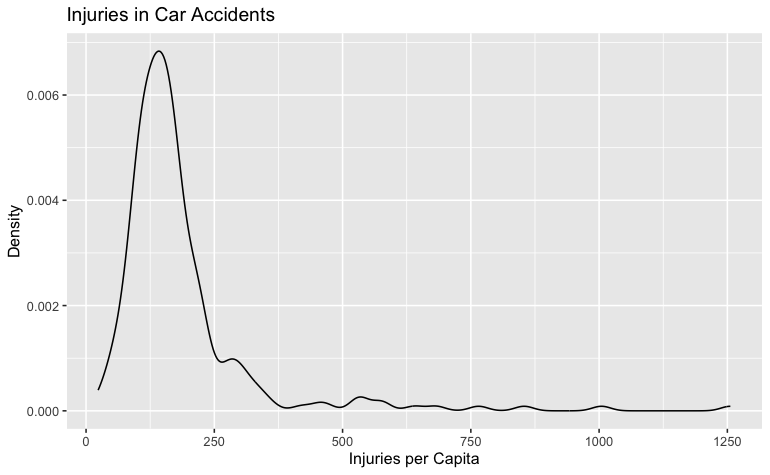
\includegraphics[width=0.8\columnwidth]{../presentation/presentation_images/injury_dist.png}
\end{center}

It seems that, on average, a county in Colorado sees approximately 150 injuries in car accidents on any given season per year per 100 thousand residents. We can also see that the distribution of injuries appears log normal. We see most values hovering between 100 and 200 with a very long right tail. As we need our response variable to be normally distributed this immediately puts a log transformation into consideration. It is worth noting that a log transformation of the response variable does complicate model interpretation slightly and so should not be done without reason.

\begin{table}[h!]
\centering
\begin{tabular}{|l|r|r|r|r|r|r|}
\hline
\rowcolor[HTML]{E7EAF6} 
\multicolumn{1}{|c|}{\textbf{}} & \multicolumn{1}{c|}{Min} & \multicolumn{1}{c|}{1st Quartile} & \multicolumn{1}{c|}{Median} & \multicolumn{1}{c|}{Mean} & \multicolumn{1}{c|}{3rd Quartile} & \multicolumn{1}{c|}{Max} \\ \hline
Untransformed & 23.55 & 116.09 & 150.63 & 183.73 & 197.19 & 1255.83 \\ \hline
Transformed & 3.159 & 4.754 & 5.015 & 5.048 & 5.284 & 7.136 \\ \hline
\end{tabular}
\caption{Numerical summary of Injuries, with and without log transformation}
\end{table}

Instead of including a plot showing the transformed variable, I feel this numerical summary will suffice. The more extreme values have been pulled inline with the rest of our data which is shown by the mean not being as far from the median. The resulting density plot also does appear far more normal though is not included here. We will look at more evidence in the structural section of this report later. 

\subsubsection*{Predictor Variable Candidates}

\begin{table}[h!]
\centering
\begin{tabular}{|l|r|r|r|r|r|r|}
\hline
\rowcolor[HTML]{E7EAF6} 
\multicolumn{1}{|c|}{\textbf{Predictor}} & \multicolumn{1}{c|}{Min} & \multicolumn{1}{c|}{1st Quartile} & \multicolumn{1}{c|}{Median} & \multicolumn{1}{c|}{Mean} & \multicolumn{1}{c|}{3rd Quartile} & \multicolumn{1}{c|}{Max} \\ \hline
Deaths & 0 & 2.10 & 4.19 & 10.71 & 9.62 & 179.40 \\ \hline
Bad Weather Accidents & 0 & 28.33 & 51.37 & 93.43 & 97.23 & 904.07 \\ \hline
Income & 34578 & 56303 & 65976 & 70543 & 85228 & 139010 \\ \hline
Commute Time & 11.80 &  17.23 & 20.05 & 21.17 & 23.27 & 42.40 \\ \hline
\end{tabular}
\caption{Numerical summary of predictor candidates.}
\end{table}



As for season, that one is set up such that each season shows up 64 times in the dataset. So I opted to not include a summary of that.

For this model we have 5 candidates predictors. When examining bivariate relationships between each predictor and the response we can already begin to guess which of these candidates will be included in the final model. Both deaths and bad weather accidents seem to have a positive linear relationship with injuries. However, neither income or commute time seem to have much of a linear relationship at all. All of these bivariate plots also included season as a dimension via color. What I saw did not seem to indicate any noticable groups based on season. I used this information to decide that I was probably going to stick to a parallel lines model to avoid additional complexity. 

As for season and injury, at first glance there didn't seem to be much of a relationship there as well. However, there are some differences. From most injuries to least we see summer at the top, followed by fall, winter and lastly is spring with the least number of injuries. Whether these differences would be substantial enough to warrant inclusion didn't seem obvious to me. 

\subsection*{Variable Selection}

I performed the variable selection process twice. First with the untransformed response and second with the transformed response. My preference in variable selection was for as simple a model as possible as I'm primarily interested in interpretation. Therefore any complexity I can avoid is worth investigating.

For the first run I looked at two different methods. First I performed a stepwise selection and second was a forward selection using the BIC statistic. I used these two methods as I felt they would result in a different number of predictors and was curious to see how different these models would look. I was mostly interested in the forward selection with BIC however as I only wanted to add predictors if it was necessary. Both models ended up being the exact same. They included bad weather accidents, deaths, season and mean commuting time. So, all the predictors but median income. The model had an adjusted r squared of approximately 0.65.

For the second process using the log transformed response I only used the forward selection with the BIC statistic. My plan was to later compare it against the full model to compare their performance. The model we got from this used season, deaths and bad weather accidents as the predictors. It's adjusted r squared was far worse than the untransformed model however, at 0.48. I don't see this as an enormous downside however as this transformation resolves some structural issues we'll discuss soon.

\subsection*{Structural Checks and Influential Observations}

\subsubsection*{Brief Tangent: Deaths as the response}

This is where things get interesting. I want to take a step away from the injuries model for a moment and return to the problem proposed at the start of this project. Originally, the deaths variable was my response. I went through a very similar methodology during the variable selection process and this is the stage where the death model ceased being a viable option. The model I got had the log of injuries and mean commuting time as predictors and the log of deaths + 1 as a response. To be frank, the log transformations in this model were desperate attempts to fix some severe issues that I was unable to figure out at first. 

\begin{center}
    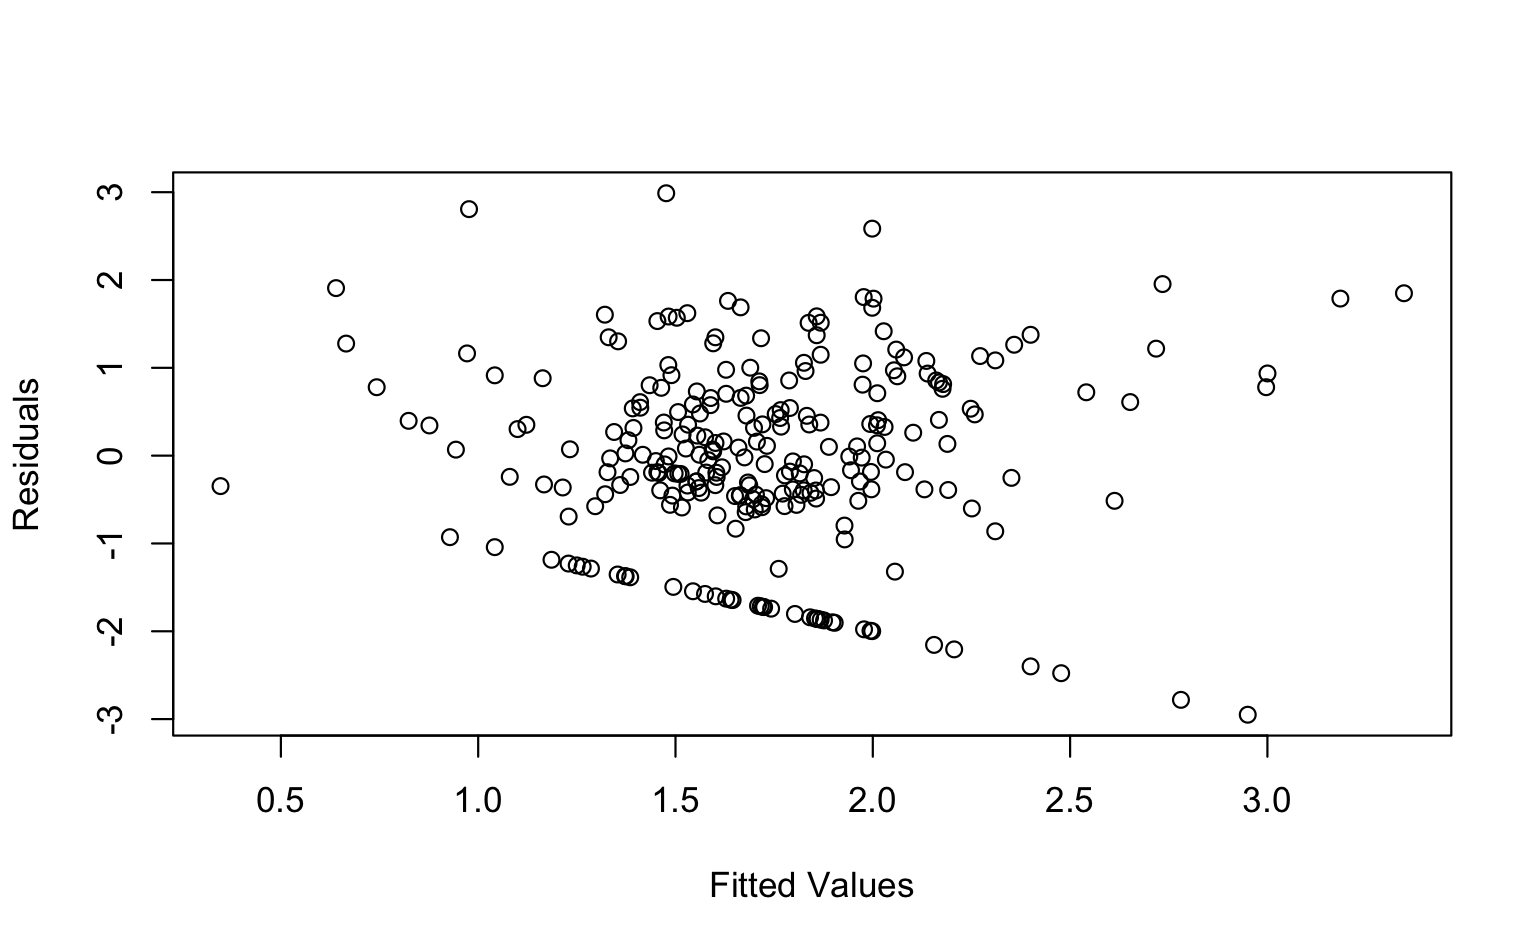
\includegraphics[width=0.7\columnwidth]{../presentation/presentation_images/deaths_residual_plot.png}
\end{center}

What we see in this residual plot is a line of values going down very consistently. Upon investigation, every single one of these points was an observation with zero deaths. About 16\% of the dataset was 0 and that resulted in a model with this trend both before and after a log transformation. 0 is a very reasonable value for the response as well so there is no justifying removal of these rows from the data. My model using deaths as a response violated some key assumptions about the errors and the results here were disasterous. This is what motivated the pivot to using injuries as the response variable. I wanted to be sure to include this aside in the report as it was the most interesting part of the process and helped inform my modeling strategy with injuries later.

What I will say is the residual plot looks fairly well behaved aside from that structural issue. I don't think linear regression is entirely useless here. One possible fix that is outside the scope of this class is to use two models. The first is a logistic regression model that assesses if the deaths response is nonzero and only then do we use a linear regression. That allows us to use the full dataset and properly handle the zeros.

\subsubsection*{Back to Injuries}

Returning to injuries, our structural checks go a lot more smoothly. I performed structural checks on both the transformed and untransformed response models. The residual plot of the untransformed model looked okay but there seemed to be some patterns in how the residuals behaved as the fitted values changed. Looking at the qq plot was also concerning as I noticed some very extreme standardized residuals at the tails. There was also noticable amounts of curving throughout the center.

As for the transformed model, things appeared to behave a lot better. Though I can't confidently claim that the errors have constant variance, the transformed model makes me far less concerned. There does seems to be a narrowing in variance as the fitted values grow more extreme however. The qq plot looks a lot better as well. There aren't any particuarly extreme values anymore and, though the plot doesn't follow the line exactly, it does follow it a lot better. This was enough evidence for me to commit to the transformed model at this point. From this point forward I completely abandon the untransformed model.

\subsubsection*{Influential Observations}

\begin{table}[h!]
\centering
\begin{tabular}{|l|r|r|r|r|r|}
\hline
\rowcolor[HTML]{E7EAF6} 
\multicolumn{1}{|c|}{\textbf{County}} & \multicolumn{1}{c|}{\textbf{Season}} & \multicolumn{1}{c|}{\textbf{Population}} & \multicolumn{1}{c|}{\textbf{Injuries per 100k/year}} & \multicolumn{1}{c|}{\textbf{Injuries per year}} \\ \hline
Mineral & Fall & 929 & 1255.8 & 11.7 \\ \hline
Mineral & Spring & 929 & 1004.7 & 9.3 \\ \hline
Hinsdale & Spring & 776 & 43.0 & 0.67 \\ \hline
\end{tabular}
\caption{Some examples of small counties.}
\end{table}


Checking for outliers gives us a few points worth considering. Index 225, 53 and 56. Using the outlier test function from the api2lm package pointed me towards index 56. This index is for Crowley county in the winter. Crowley county is a county with around 5600 people. Of note in this observation is the number of injuries at 23.55, which is both the minimum value for this variable and far below the first quantile of 116. I recommend referring back to table 2 if a refresher on the summary for injuries is needed.

Looking at leverage points brings up index 161 and 162. None of the leverage values exceed 0.30 so they don't seem to be concerning but they are still worth investigating. Looking at these rows gives us two seasons from Mineral county. Mineral county has an extremely tiny population of around 929 people. Of note in this row is the number of injuries. One row is the max for injuries at 1255, far exceeding the 3rd quantile of 197. The other row isn't far behind with a value of 1004. The thing to point out is the injuries variable is scaled by the population. Injuries really represents injuries per 100k people. The unscaled number of injuries is very small, one row has 9 injuries and the other has 12. These values just get scaled extremely high by the small population.

This happens again when we look at influential points. Mineral county comes up again but now we also get Hinsdale county which is an even smaller county with 776 people. Hinsdale in the spring has an injuries value of 43, but when we unscale that value we see this county gets less than 1 injury per year in the spring. There are a couple big takeaways from this information. First is that none of these points are so drastic that we need to remove them or handle them in any way. However these do point out a flaw in my modeling strategy. My handling for population didn't account for such small counties. It's also possible these smaller counties would be better served with a totally different type of model. Since we see such small numbers of injuries something more appropriate for discrete counts would likely perform better here.

\subsection*{Model Inference and Interpretation}

For this portion I wanted to compare my fairly simple model to the complete model and see how much performance I lose if any. To be more specific, I chose to compare the model with every predictor against a model only including deaths, season and bad weather accidents. I ran these both through a 100 fold cross validation. I chose 100 folds arbitrarily because I've never used that number before. Comparing the RMSE of the two models, they're both nearly identical with rounded values of 0.34. The MAE is similar, with the reduced model having a slightly higher value of 0.30 against 0.29 for the complete model.

These results lead me to believe that the rest of the predictiors add very little to the effectiveness of the model. I was willing to accept a decent drop in performance for the sake of interpretation but the results indicate that no such sacrifice is necessary. 

\subsubsection*{Regression Coefficients}

\begin{table}[h!]
\centering
\begin{tabular}{|l|r|r|r|r|r|}
\hline
\rowcolor[HTML]{E7EAF6} 
\textbf{Bounds} & \textbf{Spring} & \textbf{Summer} & \textbf{Winter} & \textbf{Deaths} & \textbf{Bad Weather Accidents} \\ \hline
Upper & -0.04 & 0.32 & -0.21 & 0.010 & 0.003 \\ \hline
Lower & -0.31 & 0.04 & -0.51 & 0.001 & 0.002 \\ \hline
\end{tabular}
\caption{95\% Confidence intervals for regression coefficients.}
\end{table}

\begin{table}[h!]
\centering
\begin{tabular}{|l|r|r|r|r|r|r|}
\hline
\rowcolor[HTML]{E7EAF6} 
\textbf{} & \textbf{Intercept} & \textbf{Spring} & \textbf{Summer} & \textbf{Winter} & \textbf{Deaths} & \textbf{Weather} \\ \hline
Untranslated & 4.83 & -0.18 & 0.18 & -0.36 & 0.04 & 0.003 \\ \hline
Translated & 125.87 & 0.84 & 1.20 & 0.70 & 1.004 & 1.003 \\ \hline
\end{tabular}
\caption{Regression coefficients before and after undoing log transformation.}
\end{table}


To work with these regression coefficients we need to recall that we used a log transformation on our response variable. This changes the interpretation of the regression coefficients quite a bit. You can't directly interpret -0.18 for spring as an example. What we need to do is take each coefficient, $\beta_i$, and undo the log transformation by putting it in the exponent of $e$ like $e^{\beta_i}$. From here the values give us a proportional increase or decrease of the response depending on if they're greater than or less than 1. I have the coefficients translated but I will be leaving the confidence intervals as is. As an example, if summer had a coefficient of 1.5 we would expect to see an increase in injuries of 50\% compared to the fall. If that coefficient was 0.5 we would expect to see a (1-.5) or 50\% decrease in injuries compared to the fall.  

Let us start with the intercept. We expect a typical Colorado county on any given year in the fall with 0 deaths and 0 bad weather accidents to see around 125.87 injuries per 100k people. Next up is interpreting season. I find the interpretation of this one to be a little awkward. I'm unsure if we want to compare two counties with the same $X$ values or compare the same county in two seasons. Let's assume the former despite the wording being a little awkward. Let there be two Colorado counties with the same number of deaths and bad weather accidents but one is in the fall and one is in the spring. We expect the county in the spring to see $1-0.84=16\%$ less injuries per 100k residents than the county in the fall. If that spring county was instead in the summer, we would then expect to see a $20\%$ increase in the number of injuries per 100k residents. Lastly, for winter, we would expect a $1-0.7=30\%$ decrease in the number of injuries per 100k residents compared to the fall. 

As for deaths and bad weather accidents, both have nearly identical coefficients. Let there be two Colorado counties in the same season and with the same number of bad weather accidents, however one has one additional death per 100k residents. We expect the county with the additional death to have $0.4\%$ more injuries per 100k residents. We can interpret bad weather accidents in the same vein just by flipping the wording, though we see $0.3\%$ more injuries per 100k residents instead.

Looking at the confidence intervals of our coefficients, it's a pleasant surprise to see that none of these intervals contain 0. This means that, at least at the 95\% confidence level, that 0 isn't a reasonable value for them. This is reflected in the effect plots for all of the regression coefficients as well. Deaths and bad weather accidents both show a positive relationship with injuries given the other regressors are held at their typical values. Each season also shows a meaningful difference from the other, with none of the confidence intervals seeming to overlap between the 4. All of this, combined with our other results compared against the complete model, indicate that we have a good selection of regressors. 

\subsubsection*{Collinearity}

As for collinearity, none of the predictors had VIF values that indicated an issue. The highest generalized VIF score was 1.48 for bad weather accidents. Therefore, we don't seem to have much infighting between our regressors and we can be fairly confident in the interpretation of the values that have been put forth here given the model being discussed and the data that it was fit to.